%%%%%%%%%%%%%%%%%%%%%%%%%%%%%%%%%%%%%%%%%%%%%%%%%%%%%%%%%%%%%%%%%%%%%%%%%%%%%%%%
% VPIC Gordon Bell submission 2008
%
% $LastChangedRevision$
% $LastChangedDate$
% $LastChangedBy$
%
%%%%%%%%%%%%%%%%%%%%%%%%%%%%%%%%%%%%%%%%%%%%%%%%%%%%%%%%%%%%%%%%%%%%%%%%%%%%%%%%
%\documentclass[letter,10pt]{article}
\documentclass[10pt]{article}

%%%%%%%%%%%%%%%%%%%%%%%%%%%%%%%%%%%%%%%%%%%%%%%%%%%%%%%%%%%%%%%%%%%%%%%%%%%%%%%%
% packages
%%%%%%%%%%%%%%%%%%%%%%%%%%%%%%%%%%%%%%%%%%%%%%%%%%%%%%%%%%%%%%%%%%%%%%%%%%%%%%%%
\usepackage{amsmath}
\usepackage{color}
\usepackage{latexmake}
\usepackage{setspace}
\doublespacing

%%%%%%%%%%%%%%%%%%%%%%%%%%%%%%%%%%%%%%%%%%%%%%%%%%%%%%%%%%%%%%%%%%%%%%%%%%%%%%%%
% macaros cribbed from Kevin's PoP paper
%%%%%%%%%%%%%%%%%%%%%%%%%%%%%%%%%%%%%%%%%%%%%%%%%%%%%%%%%%%%%%%%%%%%%%%%%%%%%%%%
\newcommand{\eps}{\varepsilon}
\newcommand{\vecr}{\vec{r}}
\newcommand{\vecu}{\vec{u}}
\newcommand{\vecJ}{\vec{J}}
\newcommand{\vecP}{\vec{P}}
\newcommand{\vecE}{\vec{E}}
\newcommand{\vecB}{\vec{B}}
\newcommand{\tensT}{\mathbf{T}}
\newcommand{\tensP}{\mathbf{\Pi}}
\newcommand{\tensS}{\mathbf{\Xi}}
\newcommand{\EN}{\mathcal{E}}
\newcommand{\op}{\mathcal{L}}

\newcommand{\Expect}[1]{\left< #1 \right>}
\newcommand{\Deriv}[2]{d_{#2}#1}
\newcommand{\PDeriv}[2]{\partial_{#2}#1}

\newcommand{\DotP}[2]{#1 \cdot #2}
\newcommand{\CrossP}[2]{#1 \times #2}

\newcommand{\Grad}[1]{\nabla #1}
\newcommand{\Div}[1]{\nabla \cdot #1}
\newcommand{\Curl}[1]{\nabla \times #1}

\newcommand{\Gradu}[1]{\nabla_{\vecu} #1}
\newcommand{\Divu}[1]{\nabla_{\vecu} \cdot #1}
\newcommand{\Curlu}[1]{\nabla_{\vecu} \times #1}

\newcommand{\eq}[1]{(\ref{eq:#1})}
\newcommand{\tbl}[1]{Table \ref{tbl:#1}}
\newcommand{\fig}[1]{Figure \ref{fig:#1}}

%%%%%%%%%%%%%%%%%%%%%%%%%%%%%%%%%%%%%%%%%%%%%%%%%%%%%%%%%%%%%%%%%%%%%%%%%%%%%%%%
% Brian needs macaros too 
%%%%%%%%%%%%%%%%%%%%%%%%%%%%%%%%%%%%%%%%%%%%%%%%%%%%%%%%%%%%%%%%%%%%%%%%%%%%%%%%
\newcommand{\abinitio} {\textit{ab initio}}
\newcommand{\lde}      {\lambda_{\mathrm{De}}}
\newcommand{\wpe}      {\omega_{\mathrm{pe}}}

%%%%%%%%%%%%%%%%%%%%%%%%%%%%%%%%%%%%%%%%%%%%%%%%%%%%%%%%%%%%%%%%%%%%%%%%%%%%%%%%
% add to document dimensions
% fudge if we need to add more space
%%%%%%%%%%%%%%%%%%%%%%%%%%%%%%%%%%%%%%%%%%%%%%%%%%%%%%%%%%%%%%%%%%%%%%%%%%%%%%%%
\addtolength{\topmargin}{-2cm}
\addtolength{\textheight}{6cm}
\addtolength{\oddsidemargin}{-2.25cm}
\addtolength{\evensidemargin}{-2.25cm}
\addtolength{\textwidth}{4.5cm}

%%%%%%%%%%%%%%%%%%%%%%%%%%%%%%%%%%%%%%%%%%%%%%%%%%%%%%%%%%%%%%%%%%%%%%%%%%%%%%%%
% article information
%%%%%%%%%%%%%%%%%%%%%%%%%%%%%%%%%%%%%%%%%%%%%%%%%%%%%%%%%%%%%%%%%%%%%%%%%%%%%%%%

% FIXME: CHECK AUTHOR ORDER FOR KERBYSON / BARKER
% FIXME: CHECK ABOUT TJTK
% FIXME: if we have assessment, then we need to include CCS-1 types, no? 

\title{0.37 Pflop/s and Trillion-Particle Kinetic Modeling of Laser Plasma Interaction on Roadrunner}
\author{%
K. J. Bowers\thanks{Guest Scientist, Applied Physics Divsion (X-1-PTA Plasma Theory and Applications, Presently at D.E. Shaw Research LLC, 120 W 45th Street, 39th Floor, New York, NY 10036, Email: \emph{kevin.j.bowers@gmail.com}} \and%
%
B. J. Albright\thanks{Applied Physics Division (X-1-PTA Plasma Theory and Applications), Los Alamos National Laboratory, Los Alamos, NM 87544, Email: \emph{balbright@lanl.gov}} \and%
%
B. Bergen\thanks{Computer, Computational, and Statistical Sciences Division (CCS-2 Computational Physics), Los Alamos National Laboratory, Los Alamos, NM 87544, Email: \emph{bergen@lanl.gov}} \and%
%
K. Barker\thanks{Computer, Computational, and Statistical Sciences Division (CCS-1 Computer Science on High Performance Computing), Los Alamos National Laboratory, Los Alamos, NM 87544, Email: \emph{kjbarker@lanl.gov}} \and%
%
D. Kerbyson\thanks{Computer, Computational, and Statistical Sciences Division (CCS-1 Computer Science on High Performance Computing), Los Alamos National Laboratory, Los Alamos, NM 87544, Email: \emph{djk@lanl.gov}} \and%
%
L. Yin\thanks{Applied Physics Division (X-1-PTA Plasma Theory and Applications), Los Alamos National Laboratory, Los Alamos, NM 87544, Email: \emph{lyin@lanl.gov}}}
\date{\today}

%%%%%%%%%%%%%%%%%%%%%%%%%%%%%%%%%%%%%%%%%%%%%%%%%%%%%%%%%%%%%%%%%%%%%%%%%%%%%%%%
% begin document
%%%%%%%%%%%%%%%%%%%%%%%%%%%%%%%%%%%%%%%%%%%%%%%%%%%%%%%%%%%%%%%%%%%%%%%%%%%%%%%%
\begin{document}

%%%%%%%%%%%%%%%%%%%%%%%%%%%%%%%%%%%%%%%%%%%%%%%%%%%%%%%%%%%%%%%%%%%%%%%%%%%%%%%%
% title
%%%%%%%%%%%%%%%%%%%%%%%%%%%%%%%%%%%%%%%%%%%%%%%%%%%%%%%%%%%%%%%%%%%%%%%%%%%%%%%%
\maketitle
\thispagestyle{empty}

%%%%%%%%%%%%%%%%%%%%%%%%%%%%%%%%%%%%%%%%%%%%%%%%%%%%%%%%%%%%%%%%%%%%%%%%%%%%%%%%
% abstract
%%%%%%%%%%%%%%%%%%%%%%%%%%%%%%%%%%%%%%%%%%%%%%%%%%%%%%%%%%%%%%%%%%%%%%%%%%%%%%%%
\begin{singlespace}
\begin{abstract}
We demonstrate the outstanding performance and scalability of the VPIC 
kinetic plasma modeling code on the heterogeneous IBM Roadrunner 
supercomputer at Los Alamos National Laboratory.  VPIC is a three-
dimensional, relativistic, electromagnetic, particle-in-cell code that 
self-consistently evolves a kinetic plasma.  VPIC simulations of laser 
plasma interaction (LPI) will be conducted at unprecedented fidelity 
and scale---up to $1.1 \times 10^{12}$ macro particles on as many as 
$1.3 \times 10^8$ 
computational voxels---to accurately model the particle trapping physics 
occurring within a laser-driven hohlraum in an inertial confinement 
fusion experiment.  On these calculations, sustained performance of 
0.37~Pflop/s was 
achieved.  This capability opens up the exciting possibility of using 
VPIC to model, in a first-principles manner, a problem that threatens 
the success of the multi-billion dollar DOE/NNSA National Ignition Facility.  

\vspace{2in}

\end{abstract}
\end{singlespace}

%%%%%%%%%%%%%%%%%%%%%%%%%%%%%%%%%%%%%%%%%%%%%%%%%%%%%%%%%%%%%%%%%%%%%%%%%%%%%%%%
% add break after title page
%%%%%%%%%%%%%%%%%%%%%%%%%%%%%%%%%%%%%%%%%%%%%%%%%%%%%%%%%%%%%%%%%%%%%%%%%%%%%%%%
\pagebreak

%%%%%%%%%%%%%%%%%%%%%%%%%%%%%%%%%%%%%%%%%%%%%%%%%%%%%%%%%%%%%%%%%%%%%%%%%%%%%%%%
% Introduction
%%%%%%%%%%%%%%%%%%%%%%%%%%%%%%%%%%%%%%%%%%%%%%%%%%%%%%%%%%%%%%%%%%%%%%%%%%%%%%%%
\section*{Introduction}

When a high-power laser propagates through plasma, parametric
instabilities can amplify electron and ion density fluctuations and
scatter the laser light.  Understanding these laser-plasma
instabilities (LPI) is a problem of enormous practical interest---LPI
account for half the margin for uncertainty in inertial confinement
fusion (ICF) experiments at the multi-billion-dollar National Ignition
Facility (NIF).  Indeed, demonstration of fusion ignition at the NIF
in experiments starting in 2010 requires control of LPI.

Kinetic modeling ``at scale'' using particle-in-cell kinetic plasma
simulations is the only economical and practicable means by which LPI
physics can be understood and the effects mitigated.
Large particle-in-cell plasma 
simulations typically employ tens to hundreds of millions of voxels
(cells) and a few billion simulation macroparticles (tens to hundreds
of particles/voxel).  While adequate for some problems, high levels of
noise have proved problematic for accurate modeling of the nonlinear
wave-particle kinetics of LPI~\cite{Yin_et_al_Phys_Plasmas_2006}.  The
Roadrunner hybrid petascale supercomputer (described below), however,
enables plasma kinetic modeling of LPI at unprecedented scale,
\textit{trillions of particles and billions of voxels}, which makes 
possible study of both large
simulation volume and highly intricate kinetic behavior, where
thousands of particles/voxel may be needed.  We have adapted the VPIC
kinetic plasma modeling code to run efficiently on the Roadrunner
hybrid architecture.  VPIC is a ``best in class'' explicit,
relativistic, charge-conserving, electromagnetic, particle-in-cell
code~\cite{Bowers_et_al_Phys_Plasmas_2007} developed at Los Alamos
National Laboratory and capable of simulating the physics of LPI.

This paper is structured as follows: We begin with a discussion of the
two LPI physics problems we wish to study.  Then, we describe the VPIC
kinetic plasma code.  Following this, we discuss the Roadrunner
supercomputer platform and the considerations of porting VPIC to this
platforms.  Lastly, we present measured on single-Cell chip and
extrapolated performance on up to the 12960 AMD Opteron-hosted IBM
\emph{PowerXCell 8I accelerator} chips (hereafter referred to as
``Cell'' chips).  On the full Roadrunner machine, we anticipate
sustained VPIC performance approaching 400 Tflop/s on LPI physics
problems.

%%%%%%%%%%%%%%%%%%%%%%%%%%%%%%%%%%%%%%%%%%%%%%%%%%%%%%%%%%%%%%%%%%%%%%%%%%%%%%%%
% Science
%%%%%%%%%%%%%%%%%%%%%%%%%%%%%%%%%%%%%%%%%%%%%%%%%%%%%%%%%%%%%%%%%%%%%%%%%%%%%%%%
\section{LPI in ICF Experiments}

The NIF is designed to ignite thermonuclear fuel in a laser-driven ICF
capsule, a breakthrough that will be one of the landmark achievements
in science and engineering, with a host of applications, spanning
fusion energy research, high energy density physics, and
laboratory astrophysics.  In NIF ICF experiments, which commence in
2010, 192 laser beams with 1.8~MJ of energy are directed onto the
inner walls of a hohlraum, a centimeter-sized cylindrical radiation
``bottle'' made of gold and/or uranium.  The hohlraum walls heat and
radiate x-rays, which are absorbed by a tiny ($\sim 1$~mm) capsule of
cryogenic deuterium-tritium (DT) ``fuel'' surrounded by a plastic or
beryllium ablator.  The capsule compresses to a density of hundreds of
g/cc and temperature in excess of 10~keV, conditions under which DT
fuel can ignite.

LPI jeopardize the success of fusion ignition on the NIF.  As a laser
beam travels through the plasma filling the hohlraum, it scatters from
and amplifies density irregularities.  This leads to growth of
parametric instabilities that scatter laser light and degrade energy
and symmetry of capsule compression.  The most pernicious LPI are
stimulated Raman (SRS) and Brillouin (SBS) scattering, where laser
light scatters off electron and ion density fluctuations,
respectively.

The NIF employs random phase plates to break each laser beam into a
collection of ``speckles'' or hot spots.  
%The speckle geometry depends
%on the properties of the beam, including wavelength and diffraction
%($f$/\#), and random phase plates.  
With VPIC running on the full
Roadrunner platform, we have the opportunity for the first time to
simulate \abinitio\ LPI within a solitary laser speckle under NIF-like
conditions and \textit{fully resolve} the kinetic wave-particle
dynamics.  This gives us a unique platform for understanding LPI that
will translate into improved predictive modeling of ICF experiments
and mitigation of risk for NIF ignition.

%%%%%%%%%%%%%%%%%%%%%%%%%%%%%%%%%%%%%%%%%%%%%%%%%%%%%%%%%%%%%%%%%%%%%%%%%%%%%%%%
% Science method
%%%%%%%%%%%%%%%%%%%%%%%%%%%%%%%%%%%%%%%%%%%%%%%%%%%%%%%%%%%%%%%%%%%%%%%%%%%%%%%%
\subsection{Plasma Physics Simulations}

In ICF experiments, LPI evolve to a complex, highly nonlinear state
involving wave-wave and wave-particle interaction; of greatest concern
for ignition are when wave-particle interactions dominate the
nonlinearity.  Understanding LPI under these conditions requires
high-resolution kinetic plasma simulations, as afforded by the use of
VPIC on Roadrunner, that capture all of the wave-particle physics.
These simulations must resolve complex trapped-particle orbits and
complicated structures in phase space and therefore require the use of
many simulation macroparticles (as many as thousands of
particles/voxel of each species) to resolve the
dynamics.~\cite{Yin_et_al_Phys_Plasmas_2006}

Recent experimental~\cite{Kline_PRL_2005} and
modeling~\cite{Yin_et_al_PRL_2007_SRS} work shows that LPI in a
solitary laser speckle is represented well by a diffraction-limited
laser beam.  In our three-dimensional VPIC simulations, we launch a
Gaussian diffraction-limited laser beam from a boundary into a plasma
of dimension $35 \times 6 \times 6$~$\mu$m; the simulation boundaries
absorb outgoing electromagnetic waves and reflect particles.  The
$f/4$ beam (diffraction chosen to emulate laboratory experiments and
prior calculations) is linearly polarized, of wavelength
$\lambda_0 = 351$~nm, and has peak intensity ranging from $I_0 =
10^{15} - 10^{17}$~W/cm$^2$ at the center of the simulation volume.\footnote{It 
is expected that the laser backscatter from daughter SRS and SBS waves 
is dominated by the nonlinear dynamics of the rare speckles at very 
high intensity.}
The plasma is underdense with electron density $n_e = 0.14
n_{\mathrm{cr}}$; here $n_{\mathrm{cr}} = c m_e / 2 \lambda_0 e^2$ is
the critical density, $c$ is the speed of light, $m_e$ is electron
mass, and $e$ is electronic charge (statcoul).  The simulation volume 
spans two Rayleigh lengths in $x$, the direction
of laser propagation, and three Gaussian widths of the laser
at the entrance plane in $y$ and $z$.  The electron and ion
temperatures are $T_e = 4$~keV and $T_i = 2$~keV, comparable to hohlraum
plasma conditions at maximum drive intensity.  The
hohlraum is filled with plasma comprising hydrogen, helium, and
(possibly) trace amounts of krypton and xenon.

The LPI simulations are at conditions $k \lde = 0.34$, where $k$
is the wavenumber of the most unstable electron 
fluctuation and $\lde = (k_B T_e / 4 \pi n_e e^2)^{1/2}$ is the 
Debye length ($k_B$ is Boltzmann's constant).  The simulation time is
$10^4~\wpe^{-1}$ [$\wpe = (4 \pi n_e e^2 / m_e)^{1/2}$]; 
the $1.3 \times 10^5$ time steps allow for growth
of several ``bursts'' of SRS and SBS.  The simulation volume is
divided into voxels of size $1.3 \times 1.7 \times 1.7$~Debye
lengths, which ensures ample resolution to resolve the collective
processes.

We have chosen to address two questions: (1) What is
the role is of trapped particles in the nonlinear evolution of LPI?
(2) What is the effect on LPI of high-$Z$ dopant in the
hohlraum plasma environment?

\textbf{Problem 1}
Verify recent work~\cite{Yin_et_al_PRL_2007_SRS,Yin_et_al_Phys_Plasmas_2007_SRS}
that shows that SRS and SBS saturate and are limited by nonlinear 
wave-particle trapping that bends electrostatic wavefronts (see 
Fig.~\ref{fig:lpi}), followed by transverse filamentation and break-up 
of wave fronts.  On Roadrunner, we run, for the first 
time, calculations of 1.1 trillion ($10^{12}$) simulation macroparticles,
many times larger than the next largest PIC simulations of
plasma~\cite{Yin_et_al_PRL_2007_reconnection}, to verify that 
bowing and filamentation indeed limit LPI growth.

\textbf{Problem 2}
Study the effects of high-$Z$ impurities on LPI, a proposed
LPI mitigation scheme~\cite{Lushnikov_PPCF_2006} and a problem 
arising for understanding of LPI near the hohlraum boundary (where gold 
and uranium plasma mix with the low-$Z$ gas) and ablator edge.  In 
this work, we use Kr and Xe noble gases in addition to the H and He gas
fill.  To compare with small-scale laboratory experiments of LPI, we
use a more diffracted beam ($f/3$) at higher intensity ($I_0 =
10^{17}$~W/cm$^2$). This problem requires very large numbers of
macroparticles/voxel to resolve the ion kinetics.
% FIXME: TYPO IN THIS THIS

%The early Roadrunner deployment lacks a high-performance file system,
%so our primary diagnostic for both studies is the integrated Poynting
%flux $P$ (scattered laser power) leaving the simulation volume; $P$ is
%sampled every 16 time steps and computed and output with negligible
%computational, communications, and I/O overhead.

% FIXME: CONSIDER PUTTING BACK BRIAN'S NIFTY PARAGRAPH TOWARD INTRO
%VPIC is a three-dimensional, relativistic, electromagnetic, particle-
%in-cell code ...


\begin{figure}
    \begin{center}
%    \scalebox{0.3}{\input{system.pstex_t}}
    \caption{Bowing and self-focusing of electron plasma waves from 
		a 3D SRS simulation of an f/4 speckle. Displayed are 
		isosurfaces of electron plasma waves with color 
		indicating laser field.}
    \label{fig:lpi}
    \end{center}
\end{figure}


\section{The VPIC Particle-In-Cell Code}

VPIC uses state-of-the-art techniques of relativistic plasma 
simulation~\cite{Blahovec_et_al_2000,Eastwood_et_al_1995,Jones_et_al_1996,Kwan_Snell_1985,Nieter_Cary_2004,Verboncoeur_et_al_1995}; 
these methods are briefly described below for completeness and are
further discussed in Ref.~\cite{Bowers_et_al_Phys_Plasmas_2007}.  More
in-depth analysis of PIC simulation can be found in
\cite{Birdsall_Langdon_1985,Hockney_Eastwood_1988}.

\subsection{Model Equations}

VPIC integrates the relativistic Maxwell-Boltzmann equations in a
linear background medium:
\begin{eqnarray}
\PDeriv{f_s}{t} &+& 
\DotP{c\gamma^{-1}\vecu}{\Grad{f_s}} +
\DotP{\frac{q_s}{m_s c}\left(\vecE+\CrossP{c\gamma^{-1}\vecu}{\vecB}\right)}
{\Gradu{f_s}} = \left(\PDeriv{f_s}{t}\right)_{coll} \label{eq:Boltzmann}\\
\PDeriv{\vecB}{t} &=& -\Curl{\vecE} \label{eq:Faraday}\\
\PDeriv{\vecE}{t} &=&
\eps^{-1}\Curl{\mu^{-1}\vecB} - \eps^{-1}\vecJ - \eps^{-1}\sigma\vecE
\label{eq:Ampere}
.
\end{eqnarray}
Above, $f_s\left(\vecr,\vecu,t\right)$ is the phase-space distribution
of a species $s$ with particle charge $q_s$ and mass $m_s$.  $c$ is
the speed of light in vacuum, $\vecu$ is the normalized momentum and
$\gamma\left(\vecu\right) = \sqrt{1 + u^2}$ is the relativistic
factor.  $\vecE\left(\vecr,t\right)$, $\vecB\left(\vecr,t\right)$ and
$\vecJ\left(\vecr,t\right) = \sum_s \int d\vecu q_s c\gamma^{-1}\vecu
f_s$ are electric field, magnetic field and current density.
$\eps\left(\vecr\right)$, $\mu\left(\vecr\right)$ and
$\sigma\left(\vecr\right)$ are the background diagonal permittivity,
permeability and conductivity tensors.
$\left(\PDeriv{f_s}{t}\right)_{coll}$ represents discrete particle
effects (e.g. short range Coulomb collisions, excitation and
ionization).

To avoid a costly direct discretization of $f_s$, PIC simulations
sample it with computational particles that typically represents many
physical particles.  \eq{Boltzmann} is replaced by the equations of
motion
\begin{eqnarray}
\Deriv{\vecr_{s,n}}{t} &=& c \gamma_{s,n}^{-1} \vecu_{s,n} \label{eq:Position}\\
\Deriv{\vecu_{s,n}}{t} &=& \frac{q_s}{m_s c} \left[
\vecE\left(\vecr_{s,n},t\right) +
\CrossP{c\gamma_{s,n}^{-1}\vecu_{s,n}}{\vecB\left(\vecr_{s,n},t\right)}
\right] \label{eq:Momentum}
.
\end{eqnarray}
$f_s$ for the computational particles obeys \eq{Boltzmann} outside of
discrete particle collisional effects.  A smooth $\vecJ$ is computed
from the particles for use in \eq{Faraday}-\eq{Ampere}.

\subsection{Model Discretization}

Time is discretized with an explicit 2nd order splitting of
\eq{Faraday}-\eq{Momentum} into operators that (in exact arithmetic)
can be individually applied exactly.  The result is a mixture of the
velocity Verlet, leapfrog, Boris rotation and exponential differencing
schemes
\begin{eqnarray}
\vecu_{s,n}\left(t^-\right) &=&\vecu_{s,n}\left(t-\delta_t/2\right) +
  \left(\delta_t/2\right)\vecE\left(\vecr_{s,n},t\right) \\
\vecu_{s,n}\left(t^+\right) &=&
  \textrm{Rotate}\,\vecu_{s,n}\left(t^-\right)\,\textrm{around}\,
  \vecB\left(\vecr_{s,n},t\right)\,\textrm{by}\,
  q_s\delta_t\left|\vecB\left(\vecr_{s,n},t\right)\right| /
  \left(m_s\gamma_{s,n}\right)\,\textrm{radians} \\
\vecu_{s,n}\left(t+\delta_t/2\right) &=&\vecu_{s,n}\left(t^+\right) +
  \left(\delta_t/2\right)\vecE\left(\vecr_{s,n},t\right) \\
\vecr_{s,n}\left(t+\delta_t\right) &=& \vecr_{s,n}\left(t\right) +
  c\delta_t\gamma_{s,n}\left(t+\delta_t/2\right)^{-1}
           \vecu_{s,n}\left(t+\delta_t/2\right) \\
\vecB\left(t+\delta_t/2\right) &=&
  \vecB\left(t\right) -
  \left(\delta_t/2\right)\Curl{\vecE\left(t\right)} \\
\vecE\left(t+\delta_t\right) &=&
  e^{-\delta_t\eps^{-1}\sigma}\vecE\left(t\right) +
  \eps^{-1}\left(1-e^{-\delta_t\eps^{-1}\sigma}\right)
    \left( \Curl{\mu^{-1}\vecB\left(t+\delta_t/2\right)} -
           \vecJ\left(t+\delta_t/2\right) \right) \\
\vecB\left(t+\delta_t\right) &=& \vecB\left(t+\delta_t/2\right) -
  \left(\delta_t/2\right)\Curl{\vecE\left(t+\delta_t\right)}
.
\end{eqnarray}

The simulation domain is divided into a regular mesh of identical
rectangular voxels with potentially irregular but voxel aligned
boundaries.  Because $\vecJ$ is smooth, $\vecE$, $\vecB$ and $\vecJ$
can be sampled on this mesh and interpolated between the mesh and
particles.  Particle fields are interpolated with an ``energy
conserving'' scheme; for example, $E_x$ is bilinearly interpolated
from the four Yee-mesh $E_x$ edge samples and $B_x$ is linearly
interpolated from two $B_x$ face samples of the voxel containing a
particle.  This scheme is especially efficient in simulations with
irregular boundary conditions as it uses no field samples outside the
voxel containing a particle.  Yee-mesh $\vecJ$ samples are
extrapolated from the particles by the method of Villasenor and
Buneman \cite{Villasenor_Buneman_1992}; a particle makes a $\vecJ$
contribution in each voxel through which it passes.  Though expensive,
this reduces artifacts from the accumulation of Gauss' law
($\Div{\eps\vecE}=\rho$) violations and provides efficient and robust
particle boundary interaction detection.  A variety of particle and
field boundary conditions are supported including particle absorbing,
particle reflecting, particle refluxing, perfect electric conductor,
perfect magnetic conductor, field emitting and field absorbing (first
order Higdon \cite{Higdon_1986}).

The rotation above can be done efficiently with a modified Boris push
\cite{Boris_1970}.  To avoid aliasing of cyclotron motion above the
simulation Nyquist frequency to lower frequencies, VPIC uses an
efficient energy conserving 6th order rotation angle approximation
like that in \cite{Blahovec_et_al_2000}.

The curls are computed with 2nd order finite differencing.  This and
the method of Villasenor and Buneman imply a discretized Gauss' law.
However, finite precision arithmetic error can cause small Gauss' law
violations to accumulate.  VPIC periodically applies Marder passes
\cite{Marder_1987} tuned specifically to clean these violations.
While this method is local and inexpensive, it suffices to use it
infrequently to keep this law satisfied to near machine precision.
For wavelengths comparable to the voxel dimensions, the discretized
speed of light can deviate significantly from $c$; allowing
relativistic particle motion to generate non-physical Cherenkov
radiation at these wavelengths.  VPIC uses the transverse current
adjustment method \cite{Eastwood_et_al_1995} to damp non-physical
Cherenkov radiation while leaving the discretized charge conservation
properties unchanged.

In vacuum, the field advance reduces to a basic FDTD algorithm
\cite{Yee_1966} and the time step and voxel dimensions must satisfy the
Courant condition,
$\left(c\delta_t/\delta_x\right)^2 +
 \left(c\delta_t/\delta_y\right)^2 +
 \left(c\delta_t/\delta_z\right)^2 < 1$.
Additionally, the particle advance usually requires the time
step and voxel dimensions to satisfy $\omega_p \delta_t < 2$ and
$\delta_{x,y,z}
\approx \lambda_d$ where $\omega_p$ is the peak plasma frequency and
$\lambda_d$ is the plasma Debye length
\cite{Birdsall_Langdon_1985,Hockney_Eastwood_1988}.
Given particles cannot exceed $c$, satisfying the Courant condition
and the Debye criterion is typically sufficient.  Though the time step
is stable for any cyclotron frequency, it is usually resolved for
accurate dynamics.  Sampling $f_s$ can require over thousands of
particles per voxel depending on the above and the phenomena being
studied to avoid enhanced computational particle collision rates and
resolve fully resonant kinetic phenomena.

\section{Model implementation}

%\begin{table}
%\caption{\label{tbl:Rules_of_thumb}
%VPIC implementation rules of thumb.  Data access estimates the time to
%initiate a data transfer between the processor and a level in its
%memory hierarchy.  Data movement estimates the time to move the next
%32-bits in a transfer.  Internode figures were obtained from
%benchmarks of typical high performance cluster interconnects.  The
%single precision figure corresponds to a 2.5 GHz processor completing
%a 4-vector SIMD instruction every clock.  Other rules of thumb were
%similarly extrapolated from various data sheets and benchmarks.
%Similar rules of thumb were applied in Ref.~\cite{Bowers_et_al_2006}.}
%
%\begin{center}
%\begin{tabular}{l l l c c c c}
%\hline
%\hline
%\multicolumn{3}{c}{Operation} & \hspace{18pt} & Time & \hspace{18pt} & Rel.~Cost \\
%\hline
%Data access      & \hspace{9pt} & Internode & & 10 $\mu$s & & 100,000 \\
%(Latency)        & & Memory    & & 50 ns     & & 500     \\
%                 & & L2 Cache  & & 5.0 ns    & & 50      \\
%\vspace{4pt}     & & L1 Cache  & & 1.0 ns    & & 10      \\
%Data movement    & & Internode & & 5.0 ns    & & 50      \\
%(32-bit)         & & Memory    & & 0.5 ns    & & 5       \\
%                 & & L2 Cache  & & 0.2 ns    & & 2       \\
%\vspace{4pt}     & & L1 Cache  & & 0.1 ns    & & 1       \\
%Single precision & & FLOP      & & 0.1 ns    & & 1       \\
%\hline
%\hline
%\end{tabular}
%\end{center}
%\end{table}

CPU performance has improved more rapidly than memory performance over
recent decades.  To compensate, modern CPUs use a deep memory
hierarchy with faster (though smaller and more limited) ``cache''
memories located close to the CPU.  Achieving high performance
requires minimizing latency / number of memory accesses, bandwidth /
amount of data accessed and computation, in roughly that order.
Fortunately, in most 3D parallel relativistic PIC codes, data needed
for computations on a node are spatially localized to that node or
very nearby; internode latency and bandwidth are naturally optimized.
Instead, local data motion is the dominant concern as there are
typically many particles per voxel and more field and particle data
per node than can fit in any cache.  Minimizing local data motion
requires grouping data needed to perform operations contiguously and
accessing it sequentially when possible.  As computation and storage
are cheap compared with data motion, replicating computations and/or
data is often worthwhile.

\subsection{Data motion optimization}

% SINGLE PRECISION
Single precision codes can often be made to run faster than their
double precision equivalents as single precision requires half the
data movement and most modern CPUs provide single precision 4-vector
SIMD capabilities.  For typical time steps, voxel dimensions and
particles per voxel, model discretization error exceeds single
precision arithmetic error.  Thus, single precision should usually be
acceptable provided it does not introduce non-physical artifacts
(e.g. large violations of otherwise conserved quantities).  VPIC uses
single precision to help achieve high performance but takes care to
structure operations to minimize its impact.  For example, particle
coordinates are not stored in an absolute coordinate system but as a
voxel index and offset within that voxel (interestingly, each voxel
has identical numerical properties regardless how the voxel mesh is
translated, oriented or reflected in absolute coordinates).  In
practice, single precision has not been an issue for production use of
VPIC and even more precision demanding computations have successfully
used single precision as well
\cite{Bowers_et_al_2006,Langou_et_al_2006,Lippert_et_al_2007}.
Based on extensive verification and validation studies for VPIC LPI
simulation~\cite{Yin_et_al_Phys_Plasmas_2006}, we have high confidence
that single-precision is more than adequate for this problems
described previously.

% SINGLE PASS PROCESSING
Since there is more particle data than can fit in any cache, it is
desirable to limit the number of times a particle is touched during a
time step lest performance be limited by moving particle data to and
from memory.  This can be achieved by processing the majority of the
particles in a single pass.  To further minimize the cost of moving
particle data, particle data is stored contiguously, memory aligned
and organized for 4-vector SIMD.  As a result, the inner loop streams
through particle data once using large aligned memory transfers under
the hood---the ideal memory access pattern.

% FIELD INTERPOLATION AND SORTING
Field interpolation can likewise severely impact performance.  If
particles are stored in a random order, field samples will be accessed
in a random order.  Because field samples do not fit within cache,
these accesses will often require memory transfers.  The situation is
made worse if field samples are directly accessed as several
non-contiguous memory transfers may be necessary.  Worse still is if the
field components are stored in separate arrays; in this worst case,
VPIC's field interpolation could involve up to 13 memory transfers per
particle under the hood.  Further exacerbating this, more data than
requested would be transferred as modern CPUs tend to round-up small
memory transfers to the cache line granularity.  To make field
interpolation efficient, in addition to the index+offset particle
position representation, an array of interpolation coefficients is
precomputed and saved in a contiguous, aligned, 4-vector SIMD
compatible layout.  Additionally, the particle array is periodically
sorted by the containing voxel index.  Because the particles do not
move far per time step, sorting is infrequent---every tens to hundreds
of time steps.  Nevertheless, the sorting can be done efficiently both
in-place and out-of-place in $O(N)$ operations \cite{Bowers_2001}.  As
a result, all the particles in a given voxel are processed
approximately consecutively; the interpolation coefficients necessary
for these particles will be loaded once from memory and cached.
Additionally, the interpolation coefficients themselves are accessed
approximately sequentially in large aligned transfers a near minimal
number of times.  Even though precomputing the interpolation
coefficients requires over three times the storage as the field
samples, the net impact is to reduce memory transfers to minimal
levels by making more efficient use of cache.

% FIXME: CONSIDER BRINGING THIS BACK SOMEWHAT REDUNDANT WITH OTHER
% STATEMENTS
%High temperature particle distributions generally require more
%frequent sorting to maximize overall performance than cold particle
%distributions.  Fortunately, the finite speed of light in relativistic
%simulation (or, more generally, timestep limitations due to numerical
%aliasing instabilities induced by particles moving through too many
%voxels in a step) limit the rate at which the particle array becomes
%disorganized at even the highest temperatures.  Also, the frequent
%sorting that occurs when using various particle-particle collision
%models usually eliminates the need for additional performance sorting

\subsection{SIMD optimization and exceptions}

Given single precision and SIMD compatible data layouts, all particle
processing described above is ideal for 4-vector SIMD.  However,
languages like C and FORTRAN are not expressive enough (e.g. data
alignment restrictions) to allow compilers to use 4-vector SIMD in
operations as complex as those in VPIC.  To compensate, VPIC has a C
language extension that allows portable 4-vector SIMD code to be
written and converted automatically to high performance 4-vector SIMD
instructions on a wide variety of platforms.  A similar approach was
used in \cite{Bowers_et_al_2006}.

%Consider a fairly extreme simulation with a uniform isotropic light
%species (e.g. electrons) with $\omega_p \delta_t \sim 0.2$ and
%$\delta_x \sim \lambda_d$ (by the Courant condition, the thermal
%velocity would be $\sim 0.1c$) and a heavy species (e.g. hydrogen) at
%the same temperature; only $\sim 41\%$ of light particles and $\sim
%1.1\%$ of heavy particles will cross a voxel boundary in a time step.
%(The particle representation
%requires that the coordinate system for the particle offsets need to
%be transformed when a particle crosses into a different voxel.)

Unfortunately, $\vecJ$ accumulation is not as SIMD friendly.
Determining the voxels through which a particle passed varies: one
particle might remain in the voxel in which it started while the next
might cross through several.  Fortunately, particles cross voxel
boundaries infrequently.  VPIC uses 4-vector SIMD to advance and
accumulate 4 particles at a time, assuming none of the 4 particles
cross any boundaries.  Particles that do are detected and make no
$\vecJ$ contribution during this process.  During subsequent voxel
crossing $\vecJ$ accumulation of these particles, if a particle hits
an ``exceptional'' boundary (e.g. needs to be sent to another node), the
index and remaining displacement are saved for later processing.  No
additional passes through the particles are necessary to find
exceptions.  Thus, exception handling (often slow and application
specific) is cleanly separated and does not pollute the instruction or
data caches during the particle advance.  Like the interpolation
coefficients, $\vecJ$ contributions from particle motion in a voxel
are made to a contiguous aligned set of partial currents which is then
postprocessed into $\vecJ$ prior to the field advance; the same
benefits described for interpolation coefficients apply.

\section{Roadrunner overview}

\begin{figure}
    \begin{center}
%    \scalebox{0.3}{\input{system.pstex_t}}
    \caption{Roadrunner System Overview}
    \label{fig:system}
    \end{center}
\end{figure}

The Roadrunner supercomputer, shown in Figure \ref{fig:system}, is a
hybrid, petascale system to be deployed at Los Alamos National
Laboratory in 2008.  The system is a first-of-its-kind, heterogeneous
cluster-of-clusters that utilizes a combination of 6,912, 1.8 GHz,
dual-socket, dual-core AMD Opteron \emph{host} CPUs with 12,960, 3.2
GHz, IBM \emph{PowerXCell 8I accelerator} CPU also known as the Cell
\emph{extended Double Precision (eDP)} CPU.  Each Cell eDP CPU
is capable of performing 204.8 Gflop/s single-precision (102.4 Gflop/s 
double-precision), for a total theoretical peak performance of
$2.6$~Pflop/s in single precision\footnote{The Opteron base system has 
a theoretical peak performance of $\sim$50 Tflop/s that is not included 
in this figure.}.  The Roadrunner supercomputer will be the first machine 
to achieve a sustained petaflop on the LINPACK benchmark used in ranking
the fastest supercomputers in the world for the TOP500 list
\cite{top500}.

\subsection{Connected Unit}

A Connected Unit (CU) is made up of 180 \emph{Triblade}, compute
nodes and 12 I/O nodes linked by a first-stage, 288-port Voltaire
Infiniband $4x$ DDR switch.  Using a top-down description, the
system is comprised of 18 CUs connected via eight, second-stage,
288-port Voltaire Infiniband $4x$ DDR switches.  This allows for
twelve links per CU to each of the eight switches, with 192 ports
\emph{in} and 96 ports \emph{up}, creating a 2-to-1 over-subscribed,
fat-tree network topology.  A Connected Unit is a powerful cluster in
its own right, with a theoretical peak performance of $\sim$74
Tflop/s.  A single CU of Roadrunner would rank in the top 20 on the
current (November 2007) TOP500 list.
% FIXME: IS NOVEMBER 2007 STILL CURRENT?

\subsection{Triblade}

\begin{figure}
    \begin{center}
%    \scalebox{0.2}{\input{triblade.pstex_t}}
    \caption{Triblade Compute Node}
    \label{fig:triblade}
    \end{center}
\end{figure}

A Triblade compute node, Figure \ref{fig:triblade}, actually
integrates four physical blades: one IBM LS21, dual-socket Opteron
blade, one expansion blade, and two IBM QS22 Cell blades.  The
expansion blade connects the two QS22s to the LS21 via four PCI-e $x8$
links and provides the node's ConnectX IB $4x$ DDR link to the rest of
the CU cluster.  Each PCI-e $x8$ link logically connects an Opteron
core to a Cell eDP CPU ---there is a one-to-one relationship between
Opteron cores and eDP CPUs---with a theoretical bandwidth of 2 GB/s.
%Triblades are completely diskless, running from RAM disks
%with NFS and Panasas \cite{panasas} to the LS21 only.
The LS21 blade incorporates two dual-core AMD Opteron CPUs running at
1.8 GHz with 4 GB RAM per core.  Each QS22 blade has two Cell eDP CPUs
running at 3.2 GHz with 4 GB RAM per Cell CPU.  The full Roadrunner
machine has a total of 3240 Triblade compute nodes.

\subsection{Cell Broadband Engine Architecture (CBEA)}

% FIXME: DO NOT INCLUDE UNLESS WE HAVE SPECIFIC PERMISSION BY IBM
%\begin{figure}
%    \begin{center}
%    \scalebox{0.5}{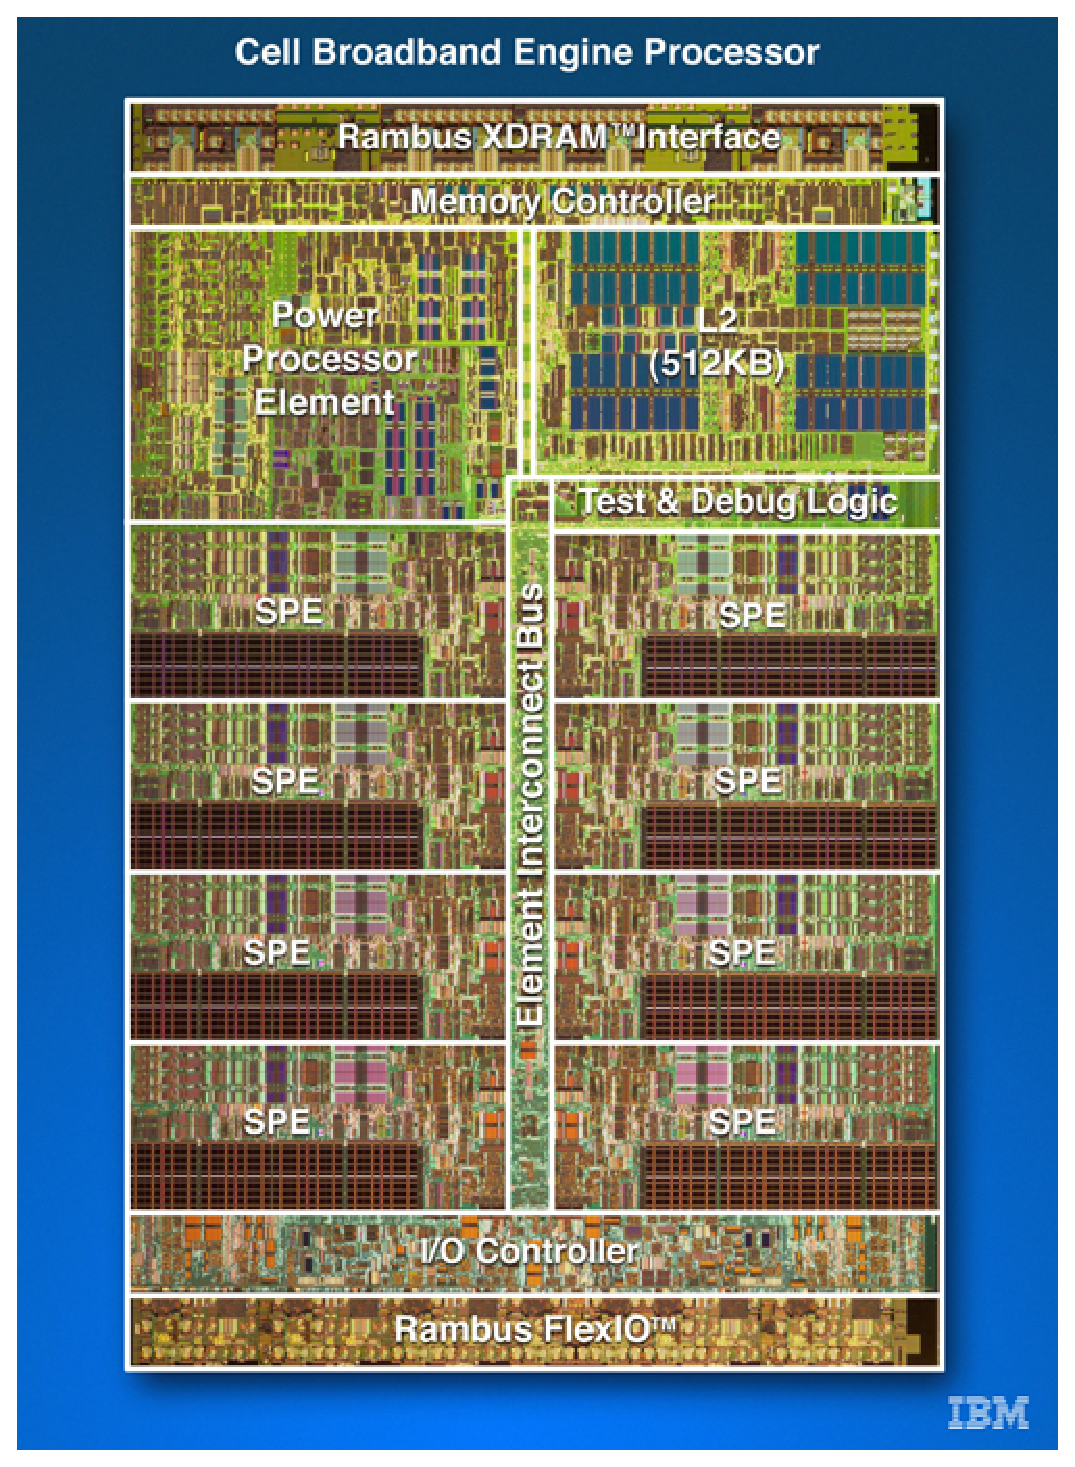
\includegraphics{cell}}
%    \caption{Cell Broadband Engine}
%    \label{image:cell}
%    \end{center}
%\end{figure}

The \emph{Cell Broadband Engine (Cell BE)}, developed jointly by Sony
Computer Entertainment, Toshiba, and IBM, is an (8+1)-way
heterogeneous parallel CPU that incorporates eight
\emph{synergistic processing elements (SPEs)} and one
\emph{power processing element (PPE)} connected via an
\emph{Element Interconnect Bus (EIB)}.  The EIB also connects
a memory controller (MIC) and two off-chip I/O interfaces.  This CPU
is used in the Sony Playstation 3 gaming console, and is currently
offered in products from IBM (QS21 blade) and Mercury Computer Systems
(CAB PCI-e card and DCBB2 blade) \cite{mercury}.  IBM has developed an
enhanced double precision version of the Cell BE chip specifically
designed for use in supercomputers like Roadrunner, the PowerXCell 8I
(Cell eDP).  Except as regards double-precision performance, the Cell
eDP does not differ significantly architecturally from the Cell BE.

The PPE is a modestly provisioned general purpose core
%capable of
%running the Linux OS, and 
which serves as a controller for the eight
SPE.  It supports two execution threads and has a theoretical peak
performance of 6.4 Gflop/s double precision at 3.2 GHz.  Each SPE core
is a 128-bit vector engine with a 256 KB user-controlled, embedded
SRAM called the \emph{Local Store (LS)}.  Additionally, each SPE has a
128-bit, 128-entry register file.  All data and text operated on by
the SPE must be fetched from main memory to the LS using \emph{direct
memory access (DMA)} calls.  Each SPE has its own 32-channel
\emph{Memory Flow Controller (MFC)} that supports up to 12 outstanding
DMA requests and has a theoretical bandwidth of 25.6 GB/s to main
memory using DDR2-800 SDRAM\footnote{The current plan of record for
Roadrunner calls for DDR2-667, in which case, the theoretical
bandwidth will be 21.4 GB/s.}.

% REDUNDANT WITH ELSEWHERE
%The Cell eDP SPEs support
%dual-issue on even and odd execution pipelines and have a theoretical
%peak performance of 204.8 Gflop/s and 102.4 Gflop/s at 3.2 GHz for
%single- and double-precision respectively.

% PROBABLY DO NOT NEED
%The EIB is configured as a four-way, circular ring with paired
%counter-rotating, uni-directional channels that are each 16 bytes
%wide.  There are currently 12 units connected to this bus, so that the
%maximum number of steps between any two units is six.  Each SPE has a
%16 byte read port and a 16 byte write port, and is capable of
%performing a read or write of 16 bytes on every EIB clock cycle.  SPEs
%are able overlap computation with communication using special DMA
%queues for requests that are still in flight.  The EIB operates at
%one-half the system clock speed and has an aggregate theoretical
%bandwidth of 204.8 GB/s at 3.2 GHz.

\section{Porting to Roadrunner}

\subsection{General strategy}

In VPIC, performance is asymptotically limited by the rate particles
can be streamed to and from DRAM.  On Roadrunner, the bandwidth
between the Cell CPU and Cell local DRAM exceeds the bandwidth between
the Cell CPU and Opteron local DRAM (limited by the PCI-Express
bridge).  However, the Cell CPU to Cell CPU bandwidth is limited by
the internode Infiniband connection.  Accordingly, in porting VPIC to
Roadrunner, we decided (1) all local simulation state would reside
within Cell DRAM, (2) the Cell CPU would be responsible for all
simulation computations and (3) the Opteron cores would manage
communications among Cell CPU.  This maximizes the bandwidth
between Cell CPU and simulation state.  It also is less complicated
to implement and allows the VPIC to be used on Cell-only clusters.

% FIXME: SOME OF THE DETAIL HERE COULD BE COMPRESSED IF SPACE IS A CONCERN
% SOME ALREADY COMPRESSED:

%(required for restart and visualization dumps).

%VPIC uses an autoconf-based build system, which supports compile-time
%selection of the target architecture.  This allows VPIC to easily be
%configured to use the original message passing abstraction layer or
%the MP Relay.  The master control logic of the code is unchanged.

%This library provides send/receive and put/get
%semantics for moving data over the PCI-e link between the LS21 and
%QS22 blades.  The interconnect between the Opteron hosts can be viewed
%as a standard flat, distributed memory topology.

%I/O requests are handled by
%double-buffered communication and calls to fread and fwrite.

To execute this strategy, we developed a message relay layer called
\emph{MP Relay} that runs on the Opterons and handles forwarding of
message traffic and remote I/O for the QS22 blades.  
%The original VPIC
%code already abstracted message passing, so this modification was
%straightforward.  
MP Relay flattens the hierarchical network
topology of Roadrunner making it possible to use the same underlying
VPIC implementation to run on Roadrunner, clusters of Cell CPU, and
traditional clusters with very little architecture specific code.  The
PPE handles communication for the Cell CPU through the abstracted
message passing layer.  Communication between Opterons and Cells is
handled within the message passing layer using the IBM \emph{Data,
Communication, and Synchronization (DaCS)} library. 
Communication among Opterons uses MPI.

% FIXME: BRING BACK IF SPACE
%In the MP Relay, message traffic is initiated by sending a DaCS
%request to the Opteron.  Send requests are followed by sending the
%actual message buffer using dacs\_send, while receive requests issue a
%dacs\_recv to accept an incoming message from the host.  On the
%Operton side, the relay runs an event loop that issues a non-blocking
%dacs\_recv call that accepts the point-to-point request data structure
%from its associated PPE peer.  Incoming requests are passed through an
%interpreter that makes additional non-blocking send (dacs\_send) and
%receive calls to complete the point-to-point communication.
%Operations that require messages to be passed to other PPEs are sent
%via MPI to that PPE's host relay, who then forwards the data to
%the PPE.

\begin{figure}
    \begin{center}
%    \scalebox{0.25}{\input{relay.pstex_t}}
    \caption{MP Relay}
    \label{fig:relay}
    \end{center}
\end{figure}

\subsection{Particle advance kernel}

Since the particle advance is the dominant cost in VPIC, it was the
focus of the initial porting efforts.  To process a particle list, the
SPE are assigned approximately equally sized non overlapping segments
of the list and their own set of partial currents to accumulate.  Each
segment contains a multiple of $16$ particles; the PPE advances any
left overs while the SPE are working.  Particle data are triple
buffered on the SPE in blocks of up to $512$ particles (at most $16$
KB are needed to hold a block---the largest size of a single DMA
transfer).  While a block is processed, the next is loaded and the
previous is stored.
%$48$ KB of local store and $3$ channels are used
%for particle triple buffering.
Block processing groups particles by $4$ and uses $4$-vector SIMD to
advance them (as done on conventional CPU).  To minimize
stalls and utilize fully the SPE's register file and dual execution
pipelines, the vectorized inner loop is hand unrolled and modulo
scheduled by $4$.  A block is guaranteed to contain a multiple
of $16$ particles, so no code is needed to process left over particles.

The challenges of SPE particle processing are handling random memory
access and particle exceptions.  Each SPE's ``local store'' is
analogous to cache, but, unlike conventional cache, memory transfers
%to and from it 
must be explicitly managed through the MFC.  Though
non-trivial, this makes it possible to design high performance
application specific cache protocols \cite{Kahle_et_al_2005}.  A $512$
line software cache of read-only interpolation coefficients, read-only
voxel adjacencies and read-write partially accumulated currents
handles random memory access.  The cache has a fully associative least
recently used (LRU) policy; a line can hold any voxel's data and the
least recently used line is replaced when caching new data.  The cache
has a simple software interface voxel\_cache\_fetch and
voxel\_cache\_wait.

voxel\_cache\_fetch initiates DMA transfers to evict the least
recently used cache line and replace it with the requested voxel's
data.  It returns the cache line where the data will be stored.
voxel\_cache\_wait waits until all pending cache DMA transfers are
complete.  Because the cache is LRU, it is easy to determine what is
cached; the last $512$ unique requests are guaranteed to be cached
after a call to voxel\_cache\_wait and before any new calls to
voxel\_cache\_fetch.  Accordingly, before block processing,
voxel\_cache\_fetch is called for each voxel referenced in the block
followed by a voxel\_cache\_wait.  Because the particle list is
approximately sorted, most of these will be cache hits.  Regardless,
the cache is large enough that, even if every particle in a block were
in different voxels, all voxel data is guaranteed to be in cache once
block processing begins.

Under the hood, voxel\_cache\_fetch queries a hash table to determine
if the requested voxel is already cached.  This hash table is
oversized to reduce collisions and uses linear probing and modular
hashing for implementation efficiency.  If a cache hit, the cache line
replacement order (stored as a doubly linked circular queue) is
updated.  If a cache miss, the least recently used line is selected
for replacement.  For read-only data, a DMA load on a channel selected
round robin from a set of channels reserved for this purpose is
initiated.  This allows multiple simultaneous fetches of read only
data.  Multiple simultaneous fetches of read-write data is more
complicated as transfers to a given voxel must not be reordered by the
MFC.  For read-write data, if the line to replace needs eviction, a
channel is selected based on the voxel's whose data is being evicted,
that data is copied to that channel's writeback buffer (first waiting
for any previous writebacks on that channel to complete) and a DMA
store is performed.  Then a fenced DMA load is initiated for the
requested read-write data on a channel selected based on the requested
voxel.  Since all transfers of read/write data to a given voxel use
the same channel, the fence is effective.  Finally, the hash table and
least recently used line are updated.  Though complicated, these
operations are a fast $O(1)$ typically.  The net impact is that minimal 
DMA transfers are used, most are overlapped and the inner
loop operates exclusively out of local store.

%Each cache line requires $268$ bytes ($192$ for the
%data, $4$ for the tag, $8$ for LRU ordering and $64$ for the hash
%table) and thus the cache requires of $134$ KB local store overall.
%$10$ channels are used for transfers of read-only data and $16$
%channels are used for transfers of read-write data.

When a particle exception occurs that the SPE logic cannot handle
(e.g. particle propagation to a neighboring node), the
particle's index and remaining displacement are saved to a list of
exceptions that occurred during block processing.  When the processed
block is stored, the list of unprocessed exceptions
%that occurred during
is streamed out to memory for later processing.

% Since up
%to $512$ exceptions could occur while processing a particle block and
%there $3$ such blocks, $24$ KB of local store and $3$ DMA channels are
%used for managing unprocessed exceptions.

Overall, $206$ KB of local store data is used for the particle advance
(leaving $50$ KB for code) and all $32$ DMA channels are utilized.
While such a strategy may seem expensive, a SPE core achieves $20\%$
of theoretical single precision peak performance and is faster
clock-for-clock than an Opteron core at the particle advance kernel
($158$ versus $174$ clocks per common case particle advance).  Further, 
the SPE cores run at a higher clock rate and there are many more of
them.  As a result, VPIC's SPE accelerated particle advance kernel can
achieve $0.517$~Pflop/s on whole of Roadrunner, over $15$ times faster
than the $0.033$~Pflop/s the kernel can achieve by running on all
Opteron cores.

\subsection{Additional porting considerations}

As shown, a kernel ported to the Cell SPE cores can deliver
outstanding performance over the Opteron cores on Roadrunner.  At the
same time, a Cell PPE core is significantly less powerful than these
Opteron cores.  Even though the parts of VPIC that run on the SPE
cores run over an order of magnitude faster than if they were run on
the Opteron cores in aggregate, the parts of VPIC that run on the PPE
cores execute $2$ to $3$ times slower!  The typical overall
simulation speed up achieved by porting VPIC from Roadrunner's
Opterons to Roadrunner's Cells is a lower (though still impressive)
$4$ to $\sim 12$, depending on simulation physical and numerical
parameters.  Thus, maximizing performance on Cell requires an
all-or-nothing porting approach.  In addition to SPE accelerating the
dominant computational kernel, other computations also need to be SPE
accelerated lest they become performance bottlenecks.  Likewise,
performance on Cell is much more sensitive to physical and numerical
parameters that affect these other computations.  In VPIC, though the
particle sort, field advance and particle exception processing are
typically negligible on conventional clusters, they are large (even
dominant in some regimes) currently when VPIC is run SPE accelerated
on Roadrunner.  Current VPIC development is focused on porting these
operations to the SPE cores.

%%%%%%%%%%%%%%%%%%%%%%%%%%%%%%%%%%%%%%%%%%%%%%%%%%%%%%%%%%%%%%%%%%%%%%%%%%%%%%%%
% Performance and Scalability
%%%%%%%%%%%%%%%%%%%%%%%%%%%%%%%%%%%%%%%%%%%%%%%%%%%%%%%%%%%%%%%%%%%%%%%%%%%%%%%%
\section{Performance and Scalability} \label{sec:performance}

This section documents methodologies used both in measuring actual
performance on the currently available hardware and in predicting the
performance that will be achieved on the full machine in June
2008.  As part of the Roadrunner deployment, two identical test
systems are available to developers in preparation for moving to the
full machine.  Each has 12 Triblade compute nodes for a total of 24 
dual-core Opterons and 48 Cell eDP CPU with a peak theoretical 
performance of 4.9 Tflop/s\footnote{This is the Cell-only performance.  
The Opterons add another 172.8 Gflop/s.}.  
%Currently, these machines are not collocated, and cannot be used as 
%a single cluster.  Access to the
%full 48 nodes of the cluster is similarly limited.  
Members of the
Performance and Architecture Team (PAL) at Los Alamos National
Laboratory were given early access to a CU at IBM's test facilities in
Poughkeepsie, New York.  This system was used to conduct some of the
scalability analysis presented here.

\subsection{Operation Count}

The operations count is dominated by the particle advance.  Within the
particle advance, the most common case is a ``cold'' particle advance,
i.e., the particle does not leave its voxel.  Cold 
advances require 246 floating point operations, obtained by hand
counting the number of % add, sub, mul, rsqrt, recip, compare, etc. 
operations in the inner loop.  The non-common case involves a particle
crossing a voxel boundary and requires an additional 168 operations plus 
168 times the number of boundaries crossed.

To estimate the total number of floating-point operations required to
push a single particle one step for a given distribution and
simulation parameters in VPIC, a random distribution of $10^7$ thermal
particles is created and advanced for one iteration.  The resulting
spatial distribution is then analyzed to estimate the probability that
a particle will cross a given number of boundaries.  The results of
this approximation are generally accurate to over 3 significant
digits, based on the assumptions that: 1) Particles are evenly
distributed in space, and 2) Particles have a drifting Maxwellian
distribution.

% FIXME: GIVE THE PROBLEM THAT THIS CORRESPONDS TO
Using this estimation with $\delta t = 0.02 \wpe^{-1}$ and voxel 
dimensions $1.3 \times 1.8 \times 1.8$ (in $\lde$), we obtain 
256.15 operations for electrons (using a thermal speed $v_{\mathrm{th}} =
1.0$), and 246.25 for ions (thermal speed reduced by
$(m_e/m_i)^{1/2}$).  These values are weighted by the fraction of 
the number of particles of each type present and averaged to obtain 
a single per particle operation count.  This estimate represents a 
lower bound because we do not include the cost of field solve or 
other bookkeeping.

\subsection{Performance on a Single Cell}

Two input decks, P1 and P2, corresponding to the two problems
identified above, were considered and used to evaluate the
single-chip performance:

\textbf{P1}:  On a single Cell CPU, a $22 \times 21 \times 21$ mesh 
is used with 1755 particles/voxel of each of five particle species.
%(This problem is more "common case'' in the ratio of particles/voxel
%than P2).  
Scaled to the full Roadrunner machine, the simulation would
use 1.1 trillion particles and 126 million voxels.  This uses
essentially all available system memory (necessitating the use of an
in-place sort).  This problem sustained 27.2 Gflop/s.

\textbf{P2}:  On a single Cell CPU, a $13 \times 14 \times 14$ mesh 
is used with 3900 particles/voxel of each of five particle species.
P2 showcases VPIC's ability to employ a very large number of
particles/voxel to resolve highly detailed phase space structures.
Scaled to the full Roadrunner machine, this problem would employ 643
billion particles and 33 million voxels. This uses essentially all
available system memory, but with an out-of-place sort for improved
sorting performance.  This problem sustained 32.2 Gflop/s.

Performance is a balance between loss of spatial locality (which
degrades software cache performance on the SPU particle advance) and
time spent sorting particles.  Generally, electrons, being the hottest
species, delocalize most rapidly and therefore need to be sorted most 
frequently.  On both problems, electron and ion sort intervals were 
optimized.  

\begin{table}
\caption{\label{tbl:ASDS_Weak_Scalability}
Weak Scalability}

\begin{center}
\begin{tabular}{l c c}
\hline
\hline
Cell Cores & Gflop/s per Core & Projected Full Machine Tflop/s Performance \\
 & & (based on this measurement) \\
\hline
1 & 32.2 & 404.3 \\
4 & 29.8 & 386.0 \\
8 & 29.1 & 377.5 \\
16 & 28.5 & 369.8 \\
36 & 28.4 & 367.5 \\
\hline
\end{tabular}
\end{center}
\end{table}

%Outline I see (BJA):  
%\begin{itemize}
%\item XXXXX Single core performance on tuned VPIC deck.
%
%\item ????? How we optimized:  large particle number; sort interval to be 
%balance between performance gain from improved data locality vs. 
%cost of doing the sort. 
%
%\item ????? Breakdown of how we infer single-core performance.  (What flops go to 
%what; worst-case, we give a lower bound on performance from cold particle
%benchmark).  What does this translate into in terms of theoretical peak 
%flops?  In terms of bandwidth to memory? 
%
%\item Summarize Kevin Barker's measured scaling on a less-particle-dominated 
%simulation.  (216 ppc on VPIC with broken earlier version of VPIC). 
%
%\item Anticipated scaling for full Roadrunner from scaling up of tuned 
%single-core measured performance (and as many as 48 cores of ASDS).  
%
%\end{itemize}

%%%%%%%%%%%%%%%%%%%%%%%%%%%%%%%%%%%%%%%%%%%%%%%%%%%%%%%%%%%%%%%%%%%%%%%%%%%%%%%%
% Conclusion
%%%%%%%%%%%%%%%%%%%%%%%%%%%%%%%%%%%%%%%%%%%%%%%%%%%%%%%%%%%%%%%%%%%%%%%%%%%%%%%%
\section{Conclusion}

VPIC has been shown to run very efficiently on the Roadrunner hybrid 
platform on problems that are particle-dominated.  Currently, 
we are SPU accelerating other parts of the VPIC algorithm, in particular, 
the particle sort and the field solve.  This will improve upon the
performance we have achieved on particle-dominated simulations as 
well as expand the class of problems on which we can expect 
large speedups.  As dicsussed earlier, by Amdahl's law, the faster the 
particle push becomes, the more important it is to accelerate the other
parts of the algorithm.  We expect to have made significant progress
towards this by the time the full Roadrunner system becomes available,
which make make accessible sustained 400+ Tflop/s simulations on the 
LPI problems presented.  

%%%%%%%%%%%%%%%%%%%%%%%%%%%%%%%%%%%%%%%%%%%%%%%%%%%%%%%%%%%%%%%%%%%%%%%%%%%%%%%%
% Acknowledgments
%%%%%%%%%%%%%%%%%%%%%%%%%%%%%%%%%%%%%%%%%%%%%%%%%%%%%%%%%%%%%%%%%%%%%%%%%%%%%%%%
\subsection*{Acknowledgments}
This work was performed under the auspices of the United States Dept. 
of Energy by the Los Alamos National Security LLC Los Alamos National
Laboratory under Contract No. DE-AC52-06NA25396.  Work supported in 
part by the Laboratory Directed Research and Development (LDRD) Program.
Document release number: LA-UR-08-2405. 


%%%%%%%%%%%%%%%%%%%%%%%%%%%%%%%%%%%%%%%%%%%%%%%%%%%%%%%%%%%%%%%%%%%%%%%%%%%%%%%%
% biliography
%%%%%%%%%%%%%%%%%%%%%%%%%%%%%%%%%%%%%%%%%%%%%%%%%%%%%%%%%%%%%%%%%%%%%%%%%%%%%%%%
\begin{singlespace}
\bibliographystyle{plain}
\bibliography{bib/gb2008,bib/vpic}
\end{singlespace}

%%%%%%%%%%%%%%%%%%%%%%%%%%%%%%%%%%%%%%%%%%%%%%%%%%%%%%%%%%%%%%%%%%%%%%%%%%%%%%%%
% end document
%%%%%%%%%%%%%%%%%%%%%%%%%%%%%%%%%%%%%%%%%%%%%%%%%%%%%%%%%%%%%%%%%%%%%%%%%%%%%%%%
\end{document}
